\documentclass[11pt,a4paper]{article}
\usepackage[margin=24mm,headheight=14pt]{geometry}
\usepackage{fontspec}
\setmainfont{texgyretermes-regular.otf}[BoldFont=texgyretermes-bold.otf,ItalicFont=texgyretermes-italic.otf,BoldItalicFont=texgyretermes-bolditalic.otf]
\setsansfont{texgyreheros-regular.otf}[BoldFont=texgyreheros-bold.otf]
\setmonofont{lmmono10-regular.otf}[Scale=0.88]
\usepackage{amsmath,amssymb,booktabs,tabularx,array,graphicx}
\usepackage{caption,float,fancyhdr,setspace,enumitem}
\usepackage[hidelinks,unicode]{hyperref}
\usepackage[numbers,sort&compress]{natbib}
\usepackage{listings}
\usepackage{microtype}
\setstretch{1.08}
\setlength{\parskip}{4pt}
\setlength{\parindent}{0pt}
\setlist{nosep,leftmargin=1.5em}
\captionsetup{font=small,labelfont=bf}
\pagestyle{fancy}
\fancyhf{}
\fancyhead[L]{\small Q10 Cache Mapping}
\fancyhead[R]{\small CEA201 · AI21B}
\fancyfoot[C]{\thepage}
\lstset{basicstyle=\ttfamily\footnotesize,breaklines=true,columns=fullflexible,frame=none,keepspaces=true}
\newcolumntype{Y}{>{\raggedright\arraybackslash}X}
\newcommand{\dai}{\textsc{DAI-v1}}
\newcommand{\KiB}{\,\mathrm{KiB}}
\hypersetup{pdftitle={An Experimental Evaluation of AI-Assisted Cache Mapping for Continuous Weighing-Station Data Streams},pdfauthor={Trương Tô Dân; Trần Châu Hoàng Nam; Dương Quốc Thịnh},pdfsubject={CEA201 research report, class AI21B}}
\title{An Experimental Evaluation of AI-Assisted Cache Mapping\\for Continuous Weighing-Station Data Streams}
\author{Trương Tô Dân \quad QE210127\\Trần Châu Hoàng Nam \quad QE210145\\Dương Quốc Thịnh \quad QE210121}
\date{31 October 2026}

\begin{document}
\hypersetup{pageanchor=false}
\begin{titlepage}
\centering
\vspace*{18mm}
{\large COMPUTER ORGANIZATION AND ARCHITECTURE\par}
\vspace{4mm}
{\large CEA201\par}
\vspace{20mm}
{\LARGE\bfseries An Experimental Evaluation of\\[3mm] AI-Assisted Cache Mapping for\\[3mm] Continuous Weighing-Station Data Streams\par}
\vspace{12mm}
{\large Research Report · Question 10\par}
\vspace{18mm}
\begin{tabular}{ll}
\toprule
\textbf{Group member} & \textbf{Student ID}\\
\midrule
Trương Tô Dân & QE210127\\
Trần Châu Hoàng Nam & QE210145\\
Dương Quốc Thịnh & QE210121\\
\bottomrule
\end{tabular}
\vspace{12mm}

{\large Class: AI21B\par}
\vfill
{\large 31 October 2026\par}
\end{titlepage}
\setcounter{page}{1}
\hypersetup{pageanchor=true}

\begin{abstract}
% COUNT-BEGIN abstract
Continuous sensor processing combines sequential acquisition with repeated access to recent samples, making cache placement sensitive to the memory access pattern. This study evaluates whether a cache mapping strategy proposed with AI assistance improves on conventional direct mapping under equal data-capacity constraints. Three candidates were proposed and critically reviewed before a static, two-way XOR-indexed design was selected and frozen. A Python trace-driven simulator compared this design with direct-mapped, two-way, and four-way conventional caches, each containing 4 KiB of data with 32-byte lines. Twenty-four synthetic traces represented sequential streams, circular buffers, moving-average processing, four-sensor interleaving, and a conflict stress pattern. Each of the 96 runs used 10,000 warmup accesses followed by 100,000 measured accesses. Automated validation comprised 28 tests and 20 trace/configuration comparisons. The AI-proposed design matched all conventional caches in measured miss rate for the first four workload families. In the stress family, its measured miss rate was zero, compared with 100\% for direct mapping; the conventional associative caches eliminated these misses only when their associativity accommodated the competing blocks. The results establish a placement-specific benefit rather than a general improvement for weighing-station streams. Synthetic inputs, fixed layouts, short sample horizons, and unmeasured hardware lookup costs limit generalization. Raw results, checksums, and replay instructions accompany the report.
% COUNT-END abstract
\end{abstract}
\textbf{Keywords:} cache mapping; XOR indexing; set associativity; sensor streams; trace-driven simulation; AI-assisted design.

\section{Introduction}
% COUNT-BEGIN introduction
Continuous weighing systems repeatedly acquire measurements, retain recent samples, and perform filtering or monitoring operations. These activities need not have the same memory behavior. Sequential acquisition may benefit primarily from spatial locality, whereas a moving average repeatedly references overlapping windows. Multiple sensor buffers may either coexist in a cache or compete for the same sets, depending on their placement in memory. Consequently, the effectiveness of a mapping strategy depends on the address stream rather than on the application label alone.

Direct mapping assigns each memory block to a single cache line. Its simplicity makes it a useful baseline, but blocks with the same index can repeatedly evict one another despite unused capacity elsewhere. Set associativity provides additional positions within a set, while alternative indexing changes which blocks compete. A fair evaluation separates these mechanisms and holds data capacity, line size, write policy, input traces, and measurement periods constant.

The research question is whether an AI-proposed mapping reduces cache misses and estimated memory-access cost for continuous weighing-station streams relative to direct mapping. The null hypothesis is that no miss-rate improvement is observed in the evaluated cases. Two additional hypotheses concern a possible benefit under conflict-heavy access and sensitivity to the workload pattern. These hypotheses are evaluated descriptively; no universal performance advantage or architectural novelty is presumed.

The study contributes a frozen AI-assisted selection process, a validated simulator for four cache organizations, and a reproducible paired experiment covering 24 synthetic traces. It distinguishes AI assistance during design from machine learning operating inside a cache controller. The principal finding is conditional: the selected XOR mapping removes the constructed stress conflicts, but provides no measured miss-rate improvement in the other workload families. The following sections review related work, describe the methodology, present results, and discuss the scope of this finding.
% COUNT-END introduction

\begin{figure}[htbp]\centering
\setlength{\unitlength}{1pt}
\begin{picture}(408,42)
\put(0,10){\framebox(90,30){\shortstack{Synthetic sensor\\address traces}}}
\put(90,25){\vector(1,0){16}}
\put(106,10){\framebox(90,30){\shortstack{Frozen cache\\configurations}}}
\put(196,25){\vector(1,0){16}}
\put(212,10){\framebox(90,30){\shortstack{Paired cache\\simulation}}}
\put(302,25){\vector(1,0){16}}
\put(318,10){\framebox(90,30){\shortstack{Misses, traffic,\\assumed AMAT}}}
\end{picture}
\caption{Evaluation flow. The same frozen input is consumed by all four cache organizations.}
\end{figure}

\section{Literature Review}
% COUNT-BEGIN literature
\subsection{Cache organization and the changing evaluation context}
Classical cache organization separates placement, identification, and replacement. Placement determines eligible locations; tags distinguish blocks sharing an index; replacement selects a resident victim when those locations are occupied. Temporal and spatial locality provide the motivation for retaining recently used or neighboring data, but neither guarantees that a particular mapping distributes an application's working set evenly. Changing an index therefore changes competition without increasing the number of data lines. This distinction provides the conceptual basis for comparing conventional direct mapping, increased associativity, and XOR indexing.

The movement from single-core to multicore processing broadens the evaluation problem. Private and shared caches introduce interference among concurrently active request streams, while bandwidth, coherence, and overlapping misses affect the consequences of an eviction. Such systems differ substantially from a single sequential trace. Recent multicore cache research is relevant to mechanisms and experimental design, but its speedups cannot be transferred directly to the present one-level sensor model. The reviewed studies span 2023--2025 and address placement, replacement, learning, and application-specific behavior.

\subsection{Alternative placement and resource accounting}
Song et al. investigate randomizing conventional set-associative caches against conflict-based side-channel attacks \cite{song2024}. Their design combines index randomization, remapping, and attack detection, with implementation on a Linux-capable Rocket-Chip platform. Its central objective is security rather than minimizing misses in sensor workloads. The relevance here is the explicit treatment of changed indexing as an architectural mechanism with implementation costs. A lightweight software expression for an index does not establish that its hardware realization has negligible delay. The present study retains a static mapping and makes no corresponding security claim.

Maya separates tag and data storage while pursuing a storage-efficient secure last-level cache \cite{bhatla2024}. This work highlights the importance of defining what an equal-resource comparison means. Equal data capacity and equal total storage are different constraints when tags, replacement state, or auxiliary structures differ. The present experiment fixes data capacity at 4 KiB and reports metadata separately. Maya's organization is not reproduced, and its reported performance is not used as a prediction for the small cache. Its methodological relevance is the need to state resource assumptions before comparing results.

SassCache uses skewed placement and security-domain-dependent indexing to mitigate contention and occupancy attacks \cite{giner2023}. Its evaluation demonstrates that placement choices must be assessed against the intended objective and workload. A mechanism motivated by isolation need not maximize hit rate. For the present research, skewed placement was considered during candidate selection, but its overlapping candidate locations and additional recency state increased implementation and verification complexity. This comparison supports examining both favorable and unfavorable access patterns instead of treating a more elaborate mapping as inherently superior. Security results remain outside the present evaluation.

\subsection{Application context and the meaning of a miss}
Tartan studies processor support for robotics and includes cache management informed by application behavior \cite{bakhshalipour2024}. Its fuzzy intra-application partitioning component changes indexing and replacement metadata. The broader processor also contains other mechanisms, so a whole-system speedup cannot be attributed solely to cache placement. The transferable principle is to relate address patterns to identifiable processing activities and to isolate contributions. Accordingly, the present workload families separately represent acquisition, buffering, filtering, and interleaving, while conventional two-way caching provides a control for the XOR candidate's associativity.

Zhu et al. introduce FLACK and FURBYS for micro-operation cache replacement \cite{zhu2025}. The distinction between an offline reference and a practical policy is particularly relevant to experimental interpretation. A reference with future information may characterize an opportunity without being implementable online. Moreover, micro-operation caches have properties that differ from fixed-size data-line caching. The present candidate uses only the current address and existing cache state; it receives neither future trace information nor an execution profile. This prevents an apparently favorable result from depending on information unavailable during ordinary access processing.

EMISSARY prioritizes instruction lines according to the consequences of their misses, rather than treating every miss as equally costly \cite{nagendra2023}. This supports distinguishing miss frequency from processor performance. Its instruction-fetch context and full-system evaluation are not equivalent to the present data-cache simulator. Nevertheless, the distinction motivates reporting traffic in addition to miss rate and treating average memory access time as a separate assumed-latency calculation. Neither a lower simulated miss rate nor faster execution of the Python program establishes a hardware speedup.

\subsection{Learning-based management and AI-assisted selection}
CHROME integrates replacement, bypassing, and prefetching through online reinforcement learning \cite{lu2024}. It illustrates how learning-based management can depend on controller state, feedback, and additional metadata. Those mechanisms address a broader optimization problem than selecting a static index before evaluation. In the present study, AI proposes and critiques candidates, while the selected controller performs no learning at runtime. This separation makes the role of AI auditable without implying that a reinforcement-learning system was implemented or that its published benefits apply to the proposed cache.

PAIC distinguishes demand and prefetch requests using separate learning-based predictors \cite{yang2023}. Its results emphasize the interaction between replacement and prefetching, and the importance of identifying the comparison baseline. An improvement relative to a baseline without prefetching cannot be interpreted as the isolated effect of a replacement change under otherwise identical conditions. The present experiment therefore disables prefetching and bypassing for every design and preserves the same write policy. Comparisons against conventional two-way caching isolate the changed set grouping more closely than comparisons against direct mapping alone.

ALPS selects cache policies over frames using compact statistical sketches \cite{shahout2024}. Although it concerns software item caching rather than processor cache lines, it provides a useful perspective on the cost of tracking access history and invoking a learned decision. Its item capacities and hit-ratio results are not converted into byte capacities or processor performance claims here. Together, these studies support a bounded research contribution: a controlled evaluation of an AI-selected static mapping in a specified synthetic context. They do not establish that AI selection guarantees improvement, nor that the selected XOR expression is a new architecture.
% COUNT-END literature

\section{Methodology}
% COUNT-BEGIN methodology
\subsection{Analysis of Key Components}
A single-level, trace-driven Python simulator models tags, valid and dirty flags, exact least-recently-used replacement, line fills, and writebacks. It does not simulate payload values, coherence, pipeline timing, or energy. Hardware validation was not undertaken because the available time and financial resources were insufficient for implementing and testing a hardware prototype. All designs contain 4,096 data bytes and 32-byte lines, use aligned four-byte accesses within a 32-bit address space, and apply write-back with write-allocate. Prefetching and bypassing are disabled. Table~\ref{tab:configs} defines the organizations. Metadata is a packed-bit estimate, not Python object memory.

Three AI-proposed candidates comprised XOR direct mapping, XOR two-way set associativity, and two-bank skewed placement. A proposal, self-critique, and final-selection sequence preceded design freeze. The selected \dai{} uses two conventional ways per set and a static XOR index. It was selected for implementability and verification rather than measured performance; no official result informed selection. Its algebraic identification and writeback rules appear in Appendix~\ref{app:design}. The same AI's critique and automated checks are not characterized as independent human review.

\begin{table}[htbp]\centering\small
\caption{Fixed cache configurations and estimated metadata.}\label{tab:configs}
\begin{tabular}{lrrlrr}\toprule
Design & Sets & Ways & Index & Data (B) & Metadata (B)\\\midrule
D0 & 128 & 1 & Conventional & 4,096 & 352\\
D1 & 64 & 2 & Conventional & 4,096 & 376\\
D2 & 32 & 4 & Conventional & 4,096 & 416\\
\dai{} & 64 & 2 & XOR & 4,096 & 376\\\bottomrule
\end{tabular}
\end{table}

\subsection{Experimental Setup}
The frozen workload specification defines 24 synthetic traces across W1--W5 (Table~\ref{tab:workloads}). Each trace contains 110,000 demand accesses: 10,000 warmup accesses followed by 100,000 measured accesses. Cache contents, dirty flags, and recency survive the transition; only counters reset. The four designs consume identical files, yielding 96 paired runs. Deterministic cases run once. Random sensor selection uses ten fixed seeds; descriptive summaries retain all seeds without inferential significance claims.

Simulator validation included 28 automated tests and 20 comparisons on five small traces across four designs. A reference model stores full block identifiers and recency lists, unlike the simulator's compressed tags and recency bits/ranks. Generator checks verify every official access against its specification and compare regenerated hashes before workload freeze. Six sampled results were replayed; one was additionally reproduced from a clean extracted source copy using the same Python environment. These checks do not constitute evaluation on another machine.

Miss rate is the primary metric. Traffic counts complete-line fills and dirty writebacks within measurement, without a final flush. Relative miss reduction is undefined when D0 has zero misses and is reported as not applicable. The separately frozen latency plan evaluates penalties of 20, 50, and 100 cycles, with a common one-cycle lookup and alternative \dai{} lookup assumptions of 1.5 and 2 cycles. These are sensitivity assumptions, not measured latencies.

\begin{align}
MR &= M/A, & T &= 32(F+W_b)\ \text{bytes},\label{eq:metrics}\\
R_{\mathrm{miss}} &= 100\frac{MR_{D0}-MR_{\mathrm{DAI}}}{MR_{D0}},\quad MR_{D0}>0,\label{eq:reduction}\\
\widehat{AMAT} &= h + MR\,p.\label{eq:amat}
\end{align}
Here $A,M,F,W_b$ denote measured accesses, misses, fills, and dirty writebacks. The penalty $p$ is additional to lookup time $h$; writeback stalls are not modeled by Equation~\ref{eq:amat}. Raw JSON records retain configurations, trace and source hashes, timings, and status. Trương Tô Dân is the designated operator and authorizing group member; Codex/Python performed execution. Evidence records retain this distinction.
% COUNT-END methodology

\begin{table}[htbp]\centering\small
\caption{Workload families. All cases use four-byte accesses and fixed, declared layouts.}\label{tab:workloads}
\begin{tabularx}{\linewidth}{l r Y}\toprule
Family & Traces & Specification\\\midrule
W1 & 2 & One-pass sequential read and write streams.\\
W2 & 3 & Read-only circular buffers of 1, 4, and 16 KiB.\\
W3 & 5 & Write a new sample, then read the newest-to-oldest window including that sample; $N=8,32,128,512,2048$; 4,096-sample ring.\\
W4 & 11 & Four contiguous 1-KiB sensor buffers; one write per selected sensor; round-robin selection and ten seeded random selections.\\
W5 & 3 & Read cycles over $K=2,4,8$ blocks separated by 4 KiB; constructed conflict stress.\\\bottomrule
\end{tabularx}
\end{table}

\section{Results}
% COUNT-BEGIN results
All 96 official runs completed successfully, with no failed runs. Each contributed 100,000 measured accesses, for 9.6 million measured accesses in total. Tables~\ref{tab:results} and~\ref{tab:traffic} were generated from the collected records. The AI-selected design matched all three conventional organizations in miss rate throughout W1--W4; its advantage over D0 appeared only in W5.

Sequential reading and writing both produced a 12.5\% miss rate for every design. W1-read transferred 400,000 bytes during measurement, whereas W1-write transferred 800,000 bytes because dirty evictions accompanied fills. Thus, equal miss rates did not imply equal traffic across read and write workloads. The 1- and 4-KiB circular buffers produced zero measured misses after warmup; the 16-KiB buffer produced 12.5\% misses for all designs.

For moving-average windows of 8, 32, 128, and 512 samples, measured miss rates were 1.389\%, 0.379\%, 0.097\%, and 0.024\%, respectively. With 2,048 samples, the rate increased to 12.537\%. These values were identical across the four organizations under the frozen layout and access order. The round-robin sensor case and every random-selection seed also produced zero measured misses. For W4-random, the mean and sample standard deviation of miss rate were both zero for each design. This describes the fixed contiguous-buffer experiment rather than uncertainty across arbitrary sensor layouts.

In W5, D0 missed on every measured access for all three block counts. Conventional two-way caching eliminated measured misses for two blocks but not for four or eight. Four-way caching eliminated them for two and four blocks but not eight. The XOR candidate eliminated measured misses in all three cases (Figure~\ref{fig:stress}), reducing traffic from D0's 3,200,000 bytes to zero during measurement. The relative miss reduction against D0 was consequently 100\%; it is not a statement about execution-time reduction.

The latency sensitivity calculation preserves this distinction. Under equal assumed lookup times, equal miss rates yield equal estimated AMAT. Raising the candidate's assumed lookup time by 0.5 or 1 cycle makes its estimate worse in W1--W4, where miss rates are equal. For W5 at a 50-cycle penalty and a two-cycle candidate lookup, D0's estimate is 51 cycles per access and the candidate's is 2. All values remain conditional on Equation~\ref{eq:amat}, without hardware timing or writeback-stall measurements.
% COUNT-END results

\begin{table}[htbp]\centering\small
\caption{Measured miss rates (\%). W4 random reports the mean of ten seeds; its sample standard deviation is zero for all designs. Other rows are deterministic cases.}\label{tab:results}
\begin{tabular}{lrrrr}\toprule
Scenario & D0 & D1 & D2 & \dai{}\\\midrule
W1 read & 12.500 & 12.500 & 12.500 & 12.500\\
W1 write & 12.500 & 12.500 & 12.500 & 12.500\\
W2 1 KiB & 0.000 & 0.000 & 0.000 & 0.000\\
W2 4 KiB & 0.000 & 0.000 & 0.000 & 0.000\\
W2 16 KiB & 12.500 & 12.500 & 12.500 & 12.500\\
W3 N8 & 1.389 & 1.389 & 1.389 & 1.389\\
W3 N32 & 0.379 & 0.379 & 0.379 & 0.379\\
W3 N128 & 0.097 & 0.097 & 0.097 & 0.097\\
W3 N512 & 0.024 & 0.024 & 0.024 & 0.024\\
W3 N2048 & 12.537 & 12.537 & 12.537 & 12.537\\
W4 even & 0.000 & 0.000 & 0.000 & 0.000\\
W4 random & 0.000 & 0.000 & 0.000 & 0.000\\
W5 K2 & 100.000 & 0.000 & 0.000 & 0.000\\
W5 K4 & 100.000 & 100.000 & 0.000 & 0.000\\
W5 K8 & 100.000 & 100.000 & 100.000 & 0.000\\
\bottomrule\end{tabular}
\end{table}

\begin{table}[htbp]\centering\small
\caption{Selected measured memory traffic (bytes). No final dirty-line flush is included.}\label{tab:traffic}
\begin{tabular}{lrr}\toprule
Scenario & D0 & \dai{}\\\midrule
W1 read & 400,000 & 400,000\\
W1 write & 800,000 & 800,000\\
W3 N8 & 88,896 & 88,896\\
W3 N2048 & 402,752 & 402,752\\
W5 K8 & 3,200,000 & 0\\
\bottomrule\end{tabular}
\end{table}

\begin{figure}[htbp]\centering
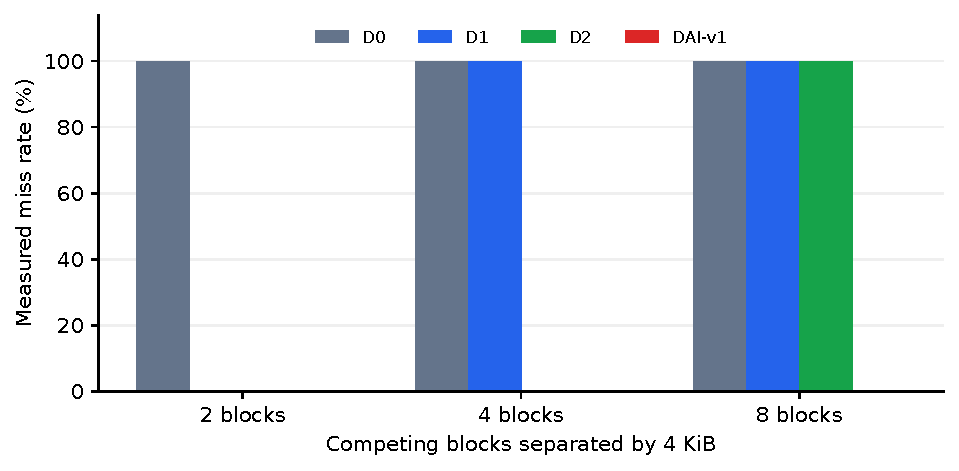
\includegraphics[width=0.94\linewidth]{figures/stress.pdf}
\caption{Measured W5 miss rates after warmup. The stress stride is known from the protocol; the result is specific to the competing-block pattern.}\label{fig:stress}
\end{figure}

\section{Discussion}
% COUNT-BEGIN discussion
The experiment supports a restricted interpretation of AI-assisted mapping. A static XOR index can remove particular direct-mapped conflicts, but AI-assisted selection did not yield a miss-rate benefit throughout the tested sensor-oriented families. This is consistent with treating mapping as a placement mechanism rather than a universal response to memory-system cost. The distinction between a useful mechanism and a broad performance claim also underlies placement and cost-aware cache research \cite{song2024,giner2023,nagendra2023}.

The W5 mechanism is directly explainable. D0 assigns blocks separated by 128 line addresses to the same line. For the selected two-way XOR index, shifting the block number mixes higher bits into the six-bit set index, dispersing the specified small group. D1 and D2 instead retain the competing group within a conventional set and are limited by their respective numbers of ways. However, the stride was known before selection and aligns with the proposed mapping. Success on this favorable stress case is a mechanism check, not evidence of general optimization or novel AI reasoning.

Several experimental choices reduce discrimination elsewhere. Contiguous sensor buffers occupy exactly 4 KiB, allowing the chosen organizations to retain the working set after warmup. Sequential streams reuse bytes within a line but not the completed lines. The frozen base alignment also avoids some adverse XOR collisions. For example, blocks 0, 65, and 130 all map to candidate set zero while occupying distinct conventional sets; a small validation counterexample demonstrates candidate misses after the conventional caches can hit. This example was not added to the official matrix after results were observed. Broader layout sensitivity remains future work.

Resource and timing trade-offs qualify the benefit. The candidate requires 376 metadata bytes under the specified packing, 24 bytes more than D0 and equal to D1. XOR logic and two tag comparisons are additional hardware considerations relative to direct mapping. Neither their area nor their delay was synthesized. As the assumed-latency results show, a lookup penalty can make unchanged miss behavior less attractive. Comparing candidate and D1 isolates set regrouping more closely; comparing candidate and D0 changes associativity and replacement as well. This distinction avoids attributing all observed differences to XOR alone \cite{bhatla2024,yang2023}.

External validity is limited by synthetic inputs, one cache capacity, one line size, no coherence or prefetching, and a fixed demand count. In W3, 110,000 accesses at $N=2048$ cover only 53 complete sampling cycles and part of another; the warmup spans only a few cycles. The measurements do not establish steady-state behavior or real-time operation. Time and budget constraints prevented hardware implementation and validation, leaving actual lookup latency, area, power, and application execution time unverified. The reference oracle and tests provide implementation evidence, but AI-assisted validation is not an independent hardware evaluation.

Future work could preregister additional alignments, longer sampling horizons, real program traces, and hardware cost models. Such experiments would retain the present batch and use separately identified inputs rather than replacing unfavorable or uninformative results. The current contribution is a reproducible controlled evaluation with an explicit negative result outside the constructed stress family.
% COUNT-END discussion

\section{Conclusion}
% COUNT-BEGIN conclusion
This study evaluated an AI-selected static XOR mapping for continuous weighing-station memory streams under a fixed 4-KiB data-capacity constraint. The selected two-way design was specified before official evaluation and compared with conventional direct-mapped, two-way, and four-way caches using the same 24 synthetic traces. Validation, frozen input hashes, raw run records, and replay checks support the traceability of the resulting 96-run experiment.

The candidate matched every conventional cache in measured miss rate across sequential streams, circular buffers, moving-average processing, and the selected four-sensor layout. Its benefit was confined to the conflict stress family: direct mapping incurred a 100\% measured miss rate, whereas the XOR candidate incurred zero after warmup for two, four, and eight competing blocks. Conventional associativity removed the conflict only when the set accommodated the group. These findings answer the research question conditionally rather than establishing a general advantage for AI-assisted design.

The candidate's additional metadata relative to direct mapping and its unmeasured lookup logic remain relevant costs. When miss rates are unchanged, an assumed lookup delay worsens estimated access time. Synthetic traces and limited sampling horizons further constrain applicability. Hardware validation was not feasible within the available time and budget. Accordingly, the evidence supports considering XOR placement for identified conflict patterns, while retaining conventional mapping as an effective baseline for the evaluated non-stress streams. Subsequent evaluation requires additional preregistered layouts, longer traces, and measured hardware costs. No claim of universal optimality, architectural novelty, or verified energy savings follows from the present results.
% COUNT-END conclusion

\clearpage
\bibliographystyle{ieeetr}
\bibliography{references}

\clearpage
\appendix
\section{Frozen Design and Implementation Details}\label{app:design}
For byte address $a$, the block number is $b=\lfloor a/32\rfloor$. A conventional cache with $S$ sets uses $s=b\bmod S$ and $t=\lfloor b/S\rfloor$. The selected candidate uses
\begin{equation}
s=(b\oplus(b\gg6))\mathbin{\&}63,\qquad t=b\gg6.
\end{equation}
Writing $b=64t+l$, with $0\le l<64$, gives $s=l\oplus(t\mathbin{\&}63)$. Consequently,
\begin{equation}
b=(t\ll6)\mathbin{|}\bigl(s\oplus(t\mathbin{\&}63)\bigr).
\end{equation}
The pair $(s,t)$ uniquely identifies a block. The victim writeback base is the recovered \emph{old} block shifted left by five, before overwriting its tag. Conventional tag/index concatenation is incorrect for this XOR mapping. Block 64, for example, has candidate index 1 and tag 1; its recovered byte base is 2,048, not 2,080.

Each access probes only the two ways of its eligible set. An invalid way is preferred, with lower way number breaking a tie. When both are valid, a one-bit exact-LRU state selects the victim; accessing or filling way $w$ makes $1-w$ least recent. A read preserves dirty state and a write sets it. Every miss fills one complete line under write-allocate; valid dirty victims produce one complete-line writeback. Invalid entries produce neither eviction nor writeback. D2 uses exact recency ranks rather than tree pseudo-LRU.

The simulator checks $H+M=A$, $M_R+M_W=M$, $F=M$, and $0\le W_b\le E\le M$ for measured counters. Invalid operations, sizes, unaligned addresses, and out-of-range addresses are rejected before state changes. Separate reset operations distinguish a new run from the transition into measurement. The model validates identity, state transitions, and traffic, not the numerical contents of sensor samples.

\section{Workload Definition and Validation}\label{app:workloads}
\begin{table}[htbp]\centering\small
\caption{Declared address layouts and generation rules. Hexadecimal values denote byte addresses.}
\begin{tabularx}{\linewidth}{l l Y}\toprule
Family & Base & Address rule\\\midrule
W1 & \texttt{0x10000000} & Access $i$ addresses base+$4i$; no wrap.\\
W2 & \texttt{0x20000000} & Address base+$4(i\bmod(B/4))$, buffer $B$ bytes; read only.\\
W3 & \texttt{0x30000000} & Cycle $q$ writes slot $q\bmod4096$, then reads slots $(q-j)\bmod4096$, $j=0,\ldots,N-1$.\\
W4 & \texttt{0x40000000} & Sensor $s$ uses base+$1024s$ plus a separate circular pointer in 256 samples; write only.\\
W5 & \texttt{0x50000000} & Address base+$4096(i\bmod K)$, $K=2,4,8$; read only.\\\bottomrule
\end{tabularx}
\end{table}

For W4-random, Python's seeded generator selects a sensor uniformly through \texttt{randrange(4)}, with seeds 1--10. W3 assumes historical samples already exist in main memory before cycle zero; the cache nevertheless starts empty. No hidden initialization access is inserted. The trace ends at the declared demand count even if this truncates a sampling cycle. The number of cache lines touched by a window depends on alignment and wrap, not merely its byte size divided by line size.

Before input freeze, every official line was checked against an access-number-based specification, separately from the generation iterator. Checks covered operation, address, access size, count, and W5's D0 index collision. Regenerated byte streams matched the stored SHA-256 values. Automated simulator tests also covered high address bits, inverse writeback, warmup preservation, exact LRU, and error handling. The following small candidate traces illustrate the expected transitions.

\begin{table}[htbp]\centering\small
\caption{Selected hand-derived expectations used in automated validation. M and H denote miss and hit.}
\begin{tabularx}{\linewidth}{Y l Y}\toprule
Trace (byte addresses) & Outcome & Additional check\\\midrule
R0, R0 & MH & One fill, no eviction.\\
R0, R2080, R0, R4160, R2080 & MMHMM & Two evictions; exact LRU.\\
W2048, R2048, R32, R4192 & MHMM & One writeback at 2048; 128 B traffic.\\
R28, R32, R28 & MMH & Distinct line boundary.\\
R0, R2080, R4160 repeated twice & MMMMMM & Candidate counterexample; D0/D1 give MMMHHH.\\\bottomrule
\end{tabularx}
\end{table}

\section{Evidence and Reproducibility}
The accompanying artifact bundle contains the source and four configurations, the 24 input traces, a trace manifest, 96 original result records, per-run and batch logs, and the analysis scripts. Each run records its input and source hashes, measurement periods, configuration snapshot, counters, and status. Raw records are retained separately from derived CSV tables and plots. The evidence index links report claims to the corresponding run ranges. No public repository or permanent artifact DOI has been assigned; the bundle is supplied with the report rather than cited as a public publication.

The pre-run snapshot records the repository HEAD and explicitly identifies uncommitted workload and tool changes. Hashes and a source archive capture those changes without assigning a fictitious commit. The evidence includes 96 successful runs and no failed runs in this batch. Six sampled replays matched counters, metrics, configurations, measurement periods, and trace hashes. One further replay matched after extracting the source snapshot into a new workspace. This verifies a clean copy within the same installed environment, not portability to an independently provisioned machine.

\begin{table}[htbp]\centering\small
\caption{Recorded execution and analysis software.}
\begin{tabular}{ll}\toprule
Component & Version / role\\\midrule
Python & 3.11.9 / simulator and generator\\
Matplotlib & 3.11.0 / figures\\
NumPy & 2.4.6 / plot preparation\\
External simulator dependencies & None; standard library only\\
\bottomrule\end{tabular}
\end{table}


AI assistance covered protocol development, candidate proposal and critique, implementation support, and report preparation. Existing prompts, responses, session records, and the design specification are preserved. They are not represented as a complete chat export. The exact AI model identifier was not available in the recorded metadata and is not inferred. Design approval and authorization to execute are attributed to Trương Tô Dân; direct execution is attributed to Codex/Python. Experimental counters originate from the simulator, not generated narrative claims.

The included replay procedure checks input and source identities before rerunning a selected record into a new output. Reproduction compares scientific fields rather than whole result-file bytes because timestamps and execution locations can change. Regeneration of traces is checked by hashes; regeneration of tables uses the frozen analysis plan.
\end{document}
